% Samsung Innovation Campus AI Course -- Capstone Project Final Report
% Compiler: XeLaTeX or LuaLaTeX; bibliography: Biber
\documentclass{sicaireport}

% ==============================================================================
% SIC-AI CAPSTONE PROJECT REPORT - METADATA CONFIGURATION
% ==============================================================================
% Fill in your team's project information below.
% This file centralizes all metadata so you do not need to edit it in multiple places.
% ==============================================================================

% Project Title
\newcommand{\projectTitle}{VietTravel AI: A Grounded Travel Assistant and Itinerary Planner for Vietnam}

% Submission Date (Format: DD/MM/YY)
\newcommand{\projectDate}{21/10/2026}

% Course & Program Information (Default)
\newcommand{\courseName}{AI Course}
\newcommand{\programName}{Samsung Innovation Campus}
\newcommand{\reportType}{Capstone Project Final Report}

% Academic Administration Information (Fixed Defaults)
\newcommand{\className}{SIC-AI-N02}
\newcommand{\instructorName}{Dr. Trần Quang Quý}

% Team Information
\newcommand{\teamName}{Travel AI Team}

% Team Members
\newcommand{\memberOne}{Nguyễn Minh Phương}
\newcommand{\memberTwo}{Thân Phú Cường}
\newcommand{\memberThree}{}
\newcommand{\memberFour}{}
\newcommand{\memberFive}{}

% Logo Path
\newcommand{\samsungLogoPath}{figures/samsung_logo.png}

% ==============================================================================
% SIC-AI CAPSTONE PROJECT REPORT - PREAMBLE CONFIGURATION
% ==============================================================================
% This file contains additional package configurations, bibliography setup,
% hyperref settings, and document-wide utility commands.
% ==============================================================================

% IEEE Bibliography via BibLaTeX
\usepackage[
    backend=bibtex,
    style=ieee,
    sorting=none,
    doi=false,
    isbn=false,
    url=true
]{biblatex}
\addbibresource{references.bib}

% Hyperref Setup with Samsung Corporate Palette
\usepackage{hyperref}
\usepackage{needspace}
\hypersetup{
    colorlinks=true,
    linkcolor=black,
    citecolor=black,
    filecolor=black,
    urlcolor=black,
    pdfauthor={\teamName},
    pdftitle={\projectTitle},
    pdfsubject={\reportType\ - \programName},
    pdfkeywords={Samsung Innovation Campus, AI Course, Capstone Project, Deep Learning, Artificial Intelligence, Multi-Agent, RAG, Tourism Recommendation}
}

% Diagrams & Visualizations
\usepackage{tikz}
\usetikzlibrary{shapes.geometric, arrows.meta, positioning, fit, calc, backgrounds}

% Algorithms & Pseudocode
\usepackage{algorithm}
\usepackage{algpseudocode}

% Additional Utility Packages
\usepackage{subcaption}
\usepackage{longtable}
\usepackage{xurl}
\usepackage{csquotes}

% Additional Utility Macros
\newcommand{\code}[1]{\texttt{#1}}
\newcommand{\abbr}[2]{\textbf{#1} (#2)}


\begin{document}
\makecoverpage
\maketitledetailpage

\pagenumbering{roman}
\setcounter{page}{1}

\chapter*{Abstract}
\addcontentsline{toc}{chapter}{Abstract}
VietTravel AI is a Flask-based travel assistant for discovering places in Vietnam and preparing one-day itinerary drafts. The repository combines a natural-language travel-search path with a separate itinerary-planning workflow. The search path detects a supported language, extracts travel-related features, queries a PostgreSQL staging table populated from OpenStreetMap (OSM), and asks a configured language-model provider to compose a response when credentials are available. The itinerary endpoint retrieves candidate points of interest (POIs), applies a deterministic schedule planner by default, checks the resulting draft against explicit identity, time, and coordinate rules, and returns the draft without saving it. A separately authenticated confirmation endpoint revalidates and persists a draft against the relational application schema.

This report documents what is present in the source tree and the accompanying data manifests. The available nationwide OSM processing summary reports 30,941 filtered candidates and 30,839 unique identifiers, although its duplicate-count fields do not reconcile exactly. The repository includes a 15-record pilot fixture and a nine-case unittest module using mocked provider and database calls. The suite was executed against the current local working tree with the project virtual environment (Python 3.10.11): all nine tests passed in 0.048 seconds. This is limited regression evidence for the tested paths, not a live database/provider evaluation. No reproducible model benchmark or load-test result is available. Accordingly, the experimental chapter separates the recorded dataset profile and passing regression run from model and system measurements that remain to be performed.

\medskip
\noindent\textbf{Keywords:} travel assistant, itinerary planning, OpenStreetMap, PostgreSQL, Flask, deterministic validation, Vietnam tourism.
\clearpage

\renewcommand{\contentsname}{Contents}
\setcounter{tocdepth}{2}
\tableofcontents
\clearpage
\listoffigures
\clearpage
\listoftables
\clearpage

\chapter*{List of Abbreviations}
\addcontentsline{toc}{chapter}{List of Abbreviations}
\begin{table}[htbp]
    \centering
    \renewcommand{\arraystretch}{1.3}
    \begin{tabularx}{\textwidth}{p{3.2cm} X}
        \toprule
        \textbf{Abbreviation} & \textbf{Definition} \\
        \midrule
        AI & Artificial intelligence \\
        API & Application programming interface \\
        CORS & Cross-origin resource sharing \\
        GPS & Global Positioning System \\
        Haversine & Great-circle distance formula for spherical coordinates \\
        HTTP & Hypertext Transfer Protocol \\
        JSON & JavaScript Object Notation \\
        JWT & JSON Web Token \\
        LLM & Large language model \\
        MAS & Multi-agent system \\
        OSM & OpenStreetMap \\
        OTP & One-time password \\
        POI & Point of interest \\
        REST & Representational State Transfer \\
        SQL & Structured Query Language \\
        SMTP & Simple Mail Transfer Protocol \\
        UI & User interface \\
        VND & Vietnamese dong \\
        \bottomrule
    \end{tabularx}
\end{table}
\clearpage

\pagenumbering{arabic}
\setcounter{page}{1}

\chapter{Introduction}
\label{chap:introduction}

\section{Background}

Travel planning brings together information that is usually scattered across maps, business listings, booking sites, public transport pages, and local recommendations. A traveler may begin with a broad question such as where to eat near a landmark, then refine it with a location, a date, a preferred pace, or a limited amount of time. A useful assistant therefore needs to do more than produce fluent text. It must retrieve places that exist, preserve their geographic identity, make the limits of incomplete information visible, and present a schedule that can be understood and changed.

This problem is especially concrete in a destination catalogue assembled from community-maintained geographic data. OpenStreetMap is a collaborative source of geographic features, and its coverage and tagging vary by place and feature type \cite{haklay2008openstreetmap}. A record can have a name and coordinates while lacking opening hours, prices, or a street address. A system that fills those gaps with plausible-sounding guesses may appear helpful while making a traveler less informed. The design challenge is thus twofold: use structured records to ground place identity, and retain explicit uncertainty where records are incomplete.

Large language models (LLMs) have made it practical to interpret open-ended questions and produce natural-language responses. Transformer models provide a flexible foundation for this interaction \cite{vaswani2017attention,brown2020language}. However, a model's linguistic fluency does not guarantee that an attraction exists, that a price is current, or that a proposed trip can be completed on time. Retrieval-augmented generation (RAG) addresses part of this problem by conditioning generation on retrieved evidence \cite{lewis2020retrieval,gao2023retrieval}. It does not, by itself, make the data current or complete, prove that the retrieval is relevant, or validate a schedule.

The repository examined in this report, \textit{ChatbotTravel\_server} (also branded in the source documentation as \textit{VietTravel AI}), is a Python web application for travel search and itinerary management. It uses Flask and Flask-RESTX to expose HTTP endpoints, SQLAlchemy to model relational data, and PostgreSQL as its intended database. A local web client is served from the same Flask application. The data pipeline prepares tourism-related points of interest (POIs) from Vietnam OSM shapefiles and loads normalized records into a PostgreSQL staging table.

There are two related but distinct interaction paths in the codebase. The travel-chat path detects language, extracts intent and features, searches the staging data, and uses configured text-generation providers when available. The itinerary path accepts a structured planning request, retrieves candidate POIs, builds a draft with a deterministic scheduling routine by default, validates it, and returns it without persistence. A separate confirmation operation checks a bearer token and persists a confirmed schedule. Keeping these paths distinct is important: the source code does not implement one autonomous graph in which every chatbot request passes through the itinerary planner.

\section{Problem Statement}

The project addresses a practical engineering question:

\begin{quote}
How can a web-based travel assistant combine conversational access to destination data with a constrained itinerary workflow while making the source and certainty of place, schedule, and route information explicit?
\end{quote}

The question decomposes into several implementation concerns:
\begin{enumerate}[leftmargin=1.8em,itemsep=4pt]
    \item \textbf{Geographic grounding.} A generated answer should use POIs retrieved from the requested geographic scope and should retain the source identifier and coordinates needed to trace a recommendation back to the catalogue.
    \item \textbf{Incomplete attributes.} Community records do not consistently contain price, rating, contact information, or opening hours. Unknown values must remain unknown rather than being silently substituted with invented values.
    \item \textbf{Schedule validity.} A generated one-day schedule needs unique stops, valid coordinates, properly formatted time intervals, no overlaps, and a reasonable upper bound on the day span. Geographic distance and actual driving time are different quantities and should not be conflated.
    \item \textbf{Persistence and identity.} A plan assembled from OSM identifiers is not automatically a record in the application's curated \code{Attractions} table. The draft and confirmation stages must preserve this distinction and verify the authenticated user before writing.
    \item \textbf{Evaluability.} A useful capstone report should separate source-code behavior, dataset manifests, and test definitions from measured model quality or runtime performance. These evidence types answer different questions.
\end{enumerate}

\section{Objectives}

The engineering objectives reflected in the inspected source tree are:
\begin{enumerate}[leftmargin=1.8em,itemsep=2pt,parsep=0pt,topsep=3pt]
    \item Provide a REST API and browser interface for travel questions and itinerary planning.
    \item Prepare Vietnam OSM data as named POIs with standardized categories, coordinates, and source metadata.
    \item Search PostgreSQL by text or category, and by radius when coordinates are available.
    \item Build one-day itinerary drafts from retrieved candidates, using the deterministic planner by default.
    \item Validate each draft in application code and report errors separately from warnings.
    \item Let verified users confirm a draft and save it transactionally.
    \item State implementation limits and propose an evaluation plan without presenting unrun experiments as results.
\end{enumerate}

\section{Scope and Non-Goals}

The report covers the contents of the repository snapshot, including the Flask entry point, application factory, controllers, service modules, ORM models, SQL migrations, data-import scripts, OSM files, the pilot JSON fixture, and the current regression-test source. The report describes the intended local development setup from \code{docker-compose.dev.yml} and \code{requirements.txt}.

The work examined here does not establish that a particular PostgreSQL instance currently contains all records described in the data manifest. It does not provide an independently labeled relevance dataset, a human evaluation panel, a reproducible load-test log, or a model-quality benchmark. The source includes optional integration code for Google Gemini in the planner and a separate provider path in the chatbot; the itinerary controller explicitly calls the planner with external API execution disabled. Consequently, the default itinerary result is produced by a deterministic heuristic rather than by a live Gemini call. The codebase also contains optional ChromaDB-related code, but the itinerary orchestrator explicitly disables it when it searches PostgreSQL.

The project should therefore be interpreted as a working prototype with implementable interfaces and validation rules, not as evidence of production-scale coverage or measured recommendation quality. In particular, a static validator can reject malformed data but cannot guarantee a correct road route, current business hours, accessibility, price, safety, or user satisfaction.

\section{Method and Evidence Policy}

This report was prepared by inspecting the repository's source files and included documentation. Its implementation claims refer to named modules and executable paths. Its dataset counts refer to \url{data/osm_full_ingestion_summary.json} and are treated as manifest values rather than a live database count. Its testing discussion describes the cases in \url{tests/test_multi_agent_flow.py} and a local run on 21 October 2026 using the project virtual environment with Python 3.10.11. All nine cases passed; database and provider calls were mocked. The result applies to the local working tree at that time and is not a live integration, model-quality, or performance benchmark.

Evidence is classified in three ways throughout the report:
\begin{description}[leftmargin=2.1cm,style=standard,itemsep=1pt,parsep=0pt]
    \item[Recorded] A value appears in a committed data file, configuration file, migration, or test definition.
    \item[Implemented] A behavior is traceable to a function or controller path in the source code.
    \item[Unmeasured] A performance, quality, or operational outcome for which the snapshot provides no reproducible run output.
\end{description}
This policy is particularly relevant to Chapter~\ref{chap:results_discussion}: the manifest provides descriptive counts, and test source provides test intentions, but neither is equivalent to an executed end-to-end benchmark.

\section{Contributions and Report Organization}

The repository's principal engineering contribution is an end-to-end structure connecting geographic data preparation to a web-facing travel application. The data loader filters and normalizes selected OSM layers; a relational staging model preserves the source identifier and source attributes; search services provide database-backed candidates; the planner produces a time-ordered draft; and a validator checks a defined set of structural and scheduling constraints. Authentication and itinerary persistence are implemented as complementary application features.

Chapter~\ref{chap:related_work} reviews recommendation, grounding, agent orchestration, and geographic planning concepts relevant to the implemented design. Chapter~\ref{chap:dataset} describes the available OSM evidence, import rules, schema, and data-quality caveats. Chapter~\ref{chap:model_configuration} explains the running architecture and its model/provider configuration. Chapter~\ref{chap:results_discussion} reports only reproducible evidence found in the repository, discusses limitations, and proposes a future evaluation protocol. Appendices provide a compact data dictionary, endpoint inventory, and the test and evaluation checklist.

\chapter{Related Work}
\label{chap:related_work}

\section{Tourism Recommender Systems}

Tourism recommendation is a context-rich decision-support problem. A traveler chooses combinations of attractions, food, accommodation, and transport under limits on place, date, time, cost, party needs, and personal interest. These decisions differ from a simple item-ranking task because the selected items form a trip: order matters, travel consumes time, and several pieces of information may be uncertain. Surveys of tourism recommenders describe content-based, collaborative, knowledge-based, and context-aware approaches as complementary families rather than a single universal solution \cite{borras2014intelligent,gavalas2014mobile}.

\subsection{Content-based and collaborative filtering}

Content-based filtering ranks items using item attributes that resemble a user's stated or learned preferences. If POIs are represented by feature vectors $\mathbf{x}_i$, and a profile by $\mathbf{u}$, a common similarity is
\begin{equation}
    \operatorname{cos}(\mathbf{u},\mathbf{x}_i)
    = \frac{\mathbf{u}^{\mathsf T}\mathbf{x}_i}
    {\lVert\mathbf{u}\rVert_2\lVert\mathbf{x}_i\rVert_2}.
\end{equation}
This family can recommend a new item if its metadata is available, but its quality depends on descriptive and consistent item features. A sparse OSM record with only a name, class, and coordinate can support category and distance filtering, but it provides little evidence about atmosphere, accessibility, or suitability for a particular traveler. The project therefore has a searchable catalogue, but the inspected implementation does not include a learned user-preference profile or a trained recommendation model.

Collaborative filtering estimates preference from interactions among users and items. In tourism settings, interactions can be sparse because many users visit a destination infrequently, and a new user or new destination may have little history. PersTour is one example: it combines POI popularity with user interests inferred from geo-tagged travel sequences and personalizes visit duration using observed photo-visit behavior \cite{lim2015persontour}. The repository's available ORM model records accounts and itineraries, but the source inspected for this report does not implement a collaborative ranking algorithm or a rating-feedback loop. It would be inaccurate to describe the current system as a trained recommender in the matrix-factorization sense.

\subsection{Context-aware and constraint-based planning}

Context-aware systems use factors such as time, location, weather, group composition, or current activity in addition to item preference \cite{gavalas2014mobile}. A travel itinerary also has hard constraints that are naturally expressed as feasibility checks: stops should not overlap, visits should fit within available hours, and locations should belong to the supported region. These constraints can be enforced independently of a language model.

An itinerary formulation can be written as the selection and ordering of a subset $\mathcal{S}$ of candidate POIs. A generalized objective may reward user relevance while penalizing time and distance:
\begin{equation}
    \max_{\mathcal{S},\pi}\;
    \sum_{i\in\mathcal{S}} u_i
    - \lambda_d\sum_{j=1}^{|\mathcal{S}|-1} d_{\pi_j,\pi_{j+1}}
    - \lambda_t\sum_{j=1}^{|\mathcal{S}|} t_{\pi_j},
\end{equation}
subject to budget, time-window, and trip-duration constraints. Here $u_i$ is an item utility, $\pi$ is the visit order, $d$ is a distance, and $t$ is a visit duration. This equation describes a useful design space; it is not the optimization objective implemented by the current planner. The current deterministic planner uses a fixed set of day-time slots and a simple dining-versus-sightseeing preference when selecting from the supplied candidate list.

\section{Large Language Models and Retrieval Grounding}

The Transformer architecture uses attention to model dependencies across sequences and underlies many contemporary language models \cite{vaswani2017attention}. Large models can interpret varied wording and generate coherent explanations, which is attractive for conversational interfaces. Few-shot language models further illustrate how prompting can guide task behavior without fitting task-specific model parameters \cite{brown2020language}. Yet a generated answer is not automatically grounded in a current local dataset. A model may confidently state a fact unsupported by the records supplied to it.
Retrieval-augmented generation combines a learned generator with external evidence retrieved at response time \cite{lewis2020retrieval}. Dense Passage Retrieval demonstrates a dual-encoder approach for retrieving passages from learned vector representations; Sentence-BERT provides a related method for producing sentence embeddings suited to semantic comparison \cite{karpukhin2020dense,reimers2019sentence}. Sparse retrieval such as BM25 provides a complementary lexical signal for exact terms \cite{robertson2009probabilistic}. A hybrid retriever can combine semantic similarity, exact text, structured category filters, and geography, but each component requires an implementation and an evaluation set. A dependency on a vector database alone does not establish that such a hybrid score is being used.

The repository contains dependencies for ChromaDB and Sentence-Transformers, and \url{poi_search_tool.py} includes an optional, read-only Chroma lookup. However, the itinerary orchestrator explicitly calls PostgreSQL search with \code{include\_chromadb=False}. Its primary retrieval path uses SQL text/category filters and, when a center coordinate and radius are supplied, geospatial filtering. The report therefore treats the itinerary flow as structured SQL retrieval, not as a deployed dense-vector RAG pipeline. In the chat path, PostgreSQL results are passed into a language-model response function; optional Google Search grounding is a separate provider capability and depends on configuration and provider availability. Search grounding does not make OSM metadata complete and cannot substitute for a domain-specific evaluation.

\section{Multi-Agent Orchestration}

Multi-agent approaches assign distinct roles to interacting language-model or software agents. Frameworks such as AutoGen and MetaGPT study communication patterns and role specialization for complex tasks \cite{wu2023autogen,hong2023metagpt}. ReAct interleaves reasoning and tool actions \cite{yao2023react}, while Reflexion introduces feedback from evaluating earlier attempts \cite{shinn2023reflexion}. These ideas motivate decomposing a travel workflow into retrieval, planning, routing, and validation responsibilities.

The itinerary workflow runs a sequence of application modules. \url{orchestrator.py} validates the request, searches staging POIs, sends candidates to the planner, checks the draft, and retries when blocking errors remain. The API controller sets \code{execute\_api=False}, so the endpoint uses the deterministic Python planner by default. A direct caller can enable the optional Gemini branch in \url{planner_agent.py} when the SDK and credentials are available; the API does not enable it.

These roles are software modules with explicit inputs and outputs, rather than concurrent autonomous agents. This structure makes each step inspectable: missing search results can be reported, unsupported OSM identifiers can be rejected, and warnings can be returned separately. The planner does not learn from user feedback, and the validator can enforce only rules that have been encoded.

\section{Geospatial Search and Route Planning}

The great-circle distance between two points on a sphere can be calculated with the Haversine formula \cite{sinnott1984virtues}. For latitudes $\phi_1,\phi_2$ and longitudes $\lambda_1,\lambda_2$ expressed in radians,
\begin{align}
    a &= \sin^2\left(\frac{\phi_2-\phi_1}{2}\right)
       + \cos(\phi_1)\cos(\phi_2)
         \sin^2\left(\frac{\lambda_2-\lambda_1}{2}\right),\\
    d &= 2R\operatorname{atan2}\left(\sqrt{a},\sqrt{1-a}\right),
\end{align}
where $R$ is an Earth-radius constant. This is a useful geographic distance, but it is not a road distance or an estimate of travel time.

The project uses this formula in two related ways. The PostgreSQL search function first applies a latitude/longitude bounding box and then evaluates Haversine distance for exact radius filtering and nearest-first ordering. The routing helper calculates direct point-to-point distance and multiplies it by a fixed factor of 1.3 to label an approximate road distance. It sets travel time to null and returns a warning; the source does not call Mapbox or OSRM for the itinerary route. This explicit uncertainty is preferable to manufacturing a drive duration, but the estimate should not be used for navigation or as proof that itinerary gaps are sufficient.
The Traveling Salesperson Problem (TSP) and Orienteering Problem provide formal models for selecting and ordering destinations under travel and time limits \cite{applegate2006traveling,vansteenwegen2011orienteering}. The repository does not implement an exact TSP solver or a road-network optimizer. Its fixed schedule slots establish temporal separation, and its route helper reports approximate distances after a draft is built. A future optimizer could combine road-network durations, opening-time windows, and explicit user utility, but would require reliable routing data and a defined objective.

\section{Open Geographic Data and Data Quality}

OpenStreetMap is a collaborative map database with uneven attribute coverage \cite{haklay2008openstreetmap}. An open extract can cover a wide area, but it is not a curated tourism catalogue. Names, category tags, addresses, and operating details depend on local mapping practices. The repository records its Vietnam OSM shapefile as an October 2026 extract under the Open Database License. The import script selects tourism-related feature classes and filters out records without names or with coordinates outside Vietnam.

Data cleaning therefore has a direct effect on system behavior. Excluding unnamed records avoids returning blank labels, while retaining null prices and hours avoids false precision. Deduplicating source identifiers is necessary when features occur in more than one shapefile layer. At the same time, a coordinate bounding box is a coarse geographic rule: it may include offshore or border-adjacent records and does not establish administrative membership. A result whose address is only a coordinate fallback remains less useful to a traveler than a verified street address.

\section{Comparison and Research Gap}

Table~\ref{tab:related_comparison} contrasts broad capability families with the evidence present in this repository. The comparison is descriptive and does not claim a controlled head-to-head experiment.

\begin{table}[htbp]
    \centering
    \caption{Capability comparison for travel-assistant design}
    \label{tab:related_comparison}
    \renewcommand{\arraystretch}{1.25}
    \begin{tabularx}{\textwidth}{>{\raggedright\arraybackslash}p{3.0cm} >{\raggedright\arraybackslash}p{4.0cm} X}
        \toprule
        \textbf{Approach} & \textbf{Strength} & \textbf{Limitation in the travel setting} \\
        \midrule
        Keyword / SQL search & Exact matching and transparent structured filters & Sensitive to wording and metadata quality; does not rank by learned preference \\
Dense vector retrieval & Can match semantically related phrasing \cite{karpukhin2020dense,reimers2019sentence} & Requires a configured embedding/index path and a relevance benchmark; absent from the default itinerary path \\
        LLM-only response & Flexible natural-language interaction \cite{brown2020language} & May state unsupported or outdated place facts; does not enforce schedule constraints by itself \\
        Retrieval-grounded generation & Conditions text generation on retrieved evidence \cite{lewis2020retrieval} & Quality depends on retrieval recall, source freshness, and faithful use of evidence \\
        Constraint validator & Reproducible rejection of defined invalid states & Cannot verify rules that are not represented, such as live traffic, budget arithmetic, or all opening-hour formats \\
        Project itinerary workflow & SQL candidate retrieval, deterministic schedule, checks, draft/confirm boundary & Does not include measured ranking quality or live road-time optimization in the inspected path \\
        \bottomrule
    \end{tabularx}
\end{table}

The engineering gap addressed by the repository is not that existing systems lack conversational or geographic features in general. Rather, it is the integration challenge of connecting a local geographic dataset, a web interface, a draft-generation flow, explicit validation, and authenticated persistence while preserving the distinction between known values and estimates. The main research opportunity is to evaluate whether this integration improves grounded usefulness and schedule feasibility under realistic Vietnamese travel queries. The available snapshot establishes implementable mechanisms and initial test scenarios, but it does not yet answer that empirical question.

\chapter{Dataset and Pre-processing}
\label{chap:dataset}

\section{Data Sources and Scope}

The main geographic source is a Vietnam extract distributed as OSM shapefiles. The local README identifies it as a Geofabrik Vietnam package obtained in October 2026 and describes the files as derived from OpenStreetMap under the Open Database License. This month and year are reported as source provenance; they do not imply that the extract is current or the latest available version.

The import script, \code{scripts/import\_all\_osm\_poi.py}, processes three layers:
\begin{itemize}[leftmargin=1.8em,itemsep=3pt]
    \item \code{gis\_osm\_pois\_free\_1}, containing named points such as restaurants, cafes, hotels, and tourism features;
    \item \code{gis\_osm\_pofw\_free\_1}, containing places of worship;
    \item \code{gis\_osm\_natural\_free\_1}, containing selected named natural features.
\end{itemize}
The source files also include administrative boundaries, roads, railways, waterways, buildings, and other layers, but the full POI importer limits ingestion to the three layers above. This reduces irrelevant records for the travel catalogue and keeps the main import process focused.

The repository also contains \code{data/osm\_vietnam\_pilot\_sample.json}, a small 15-record fixture used by the regression tests. It has five observed categories, including restaurants, cafes, hotels, Buddhist temples, and mountain attractions. It is a deterministic sample for offline planning behavior, not a representative statistical sample of the national dataset.

\section{Candidate Filtering and Standardization}

The importer's allow-list maps OSM feature classes (\code{fclass}) into user-facing categories and broader groups. It includes dining and lodging features as well as attractions, parks, museums, places of worship, memorials, and selected natural features. The filter removes records without a display name, feature classes outside the allow-list, and coordinates outside the configured Vietnam bounding box. The implemented bounds are latitude $8.0^\circ$ to $24.0^\circ$ and longitude $102.0^\circ$ to $110.0^\circ$. These bounds are a pragmatic rectangle, not an administrative-boundary polygon.

For a retained record, the importer preserves the source layer, OSM identifier, OSM class and numeric code, name, coordinates, raw properties, and tags. It creates a standardized category and summary description. If no usable address is present, the configured fallback is the explicit Vietnamese text \textit{Chưa có địa chỉ cụ thể; dùng tọa độ OpenStreetMap}. Unknown price, rating, opening hours, phone number, and image URL remain null. These choices preserve data provenance and avoid converting missing information into fabricated facts.

The import command defaults to an analytical dry run; the \code{--apply} option enables database writes. Batch size is configurable, with the documented default of 1,000. The staging table enforces a unique OSM identifier, and the importer uses an upsert strategy keyed by \code{osm\_id} to update an existing source record or insert a new one. The migration defines JSONB columns for tags, aliases, and raw properties, which allows source detail to be retained without flattening every OSM attribute into a separate relational column.

The transformation path can be summarized as a sequence of source-preserving filters. Figure~\ref{fig:poi_ingestion_pipeline} reflects the importer defaults: database writes occur only when \code{--apply} is supplied.

\begin{figure}[htbp]
    \centering
    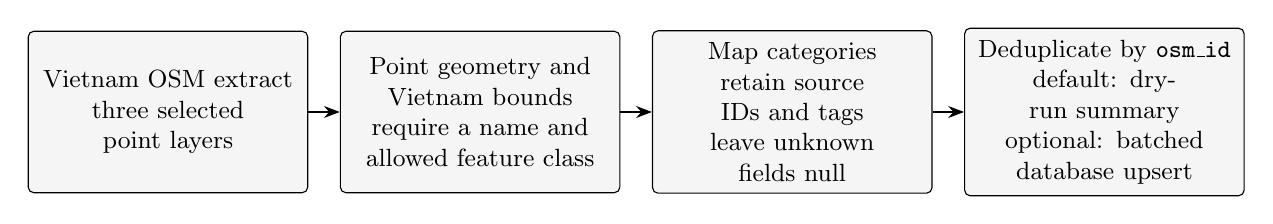
\begin{tikzpicture}[
        databox/.style={draw=black, fill=black!4, rounded corners=2pt,
            align=center, text width=3.25cm, minimum height=2.05cm,
            inner sep=1.5mm, font=\small},
        dataflow/.style={-{Stealth[length=2mm]}, thick, draw=black},
        node distance=4mm
    ]
        \node[databox] (source) {Vietnam OSM extract\\three selected point layers};
        \node[databox, right=of source] (filter) {Point geometry and Vietnam bounds\\require a name and allowed feature class};
        \node[databox, right=of filter] (normalize) {Map categories\\retain source IDs and tags\\leave unknown fields null};
        \node[databox, right=of normalize] (load) {Deduplicate by \code{osm\_id}\\default: dry-run summary\\optional: batched database upsert};
        \draw[dataflow] (source) -- (filter);
        \draw[dataflow] (filter) -- (normalize);
        \draw[dataflow] (normalize) -- (load);
    \end{tikzpicture}
    \caption{Code-derived workflow for filtering and loading geographic POIs}
    \label{fig:poi_ingestion_pipeline}
\end{figure}

\section{Recorded Dataset Profile}

The committed file \code{data/osm\_full\_ingestion\_summary.json} is the source for the descriptive profile in this section. It records 30,941 filtered candidates and 30,839 unique identifiers. Its layer-level figures and rejection counts are reproduced in Table~\ref{tab:osm_layer_profile}. These are processing-summary values; they are not a live query of the database.

\begin{table}[htbp]
    \centering
    \caption{Layer-level filtering values recorded in the ingestion summary}
    \label{tab:osm_layer_profile}
    \renewcommand{\arraystretch}{1.2}
    \small
    \setlength{\tabcolsep}{3.5pt}
    \begin{tabularx}{\textwidth}{>{\raggedright\arraybackslash}X r r r r r}
        \toprule
        \textbf{Source layer} & \textbf{Input} & \textbf{Candidates} & \textbf{No name} & \textbf{Class} & \textbf{Coords} \\
        \midrule
        OSM POIs & 75,037 & 28,482 & 23,862 & 22,678 & 15 \\
        Places of worship & 1,375 & 1,127 & 248 & 0 & 0 \\
        Natural features & 34,009 & 1,332 & 32,596 & 81 & 0 \\
        \midrule
        \textbf{Total} & \textbf{110,421} & \textbf{30,941} & \textbf{56,706} & \textbf{22,759} & \textbf{15} \\
        \bottomrule
    \end{tabularx}
\end{table}
The category-group totals in the same file sum to 30,839, as shown in Table~\ref{tab:osm_group_profile}. The distribution is concentrated in food and accommodation categories. A high count of a category does not imply high quality or completeness: it is simply a count of classified identifiers in the summary.

\begin{table}[htbp]
    \centering
    \caption{Unique POI counts by standardized category group}
    \label{tab:osm_group_profile}
    \renewcommand{\arraystretch}{1.2}
    \begin{tabularx}{0.78\textwidth}{>{\raggedright\arraybackslash}X r r}
        \toprule
        \textbf{Category group} & \textbf{Records} & \textbf{Share} \\
        \midrule
        Food and dining & 18,317 & 59.40\% \\
        Lodging & 6,454 & 20.92\% \\
        Tourism & 2,082 & 6.75\% \\
        Nature & 1,311 & 4.25\% \\
        Spiritual places & 1,129 & 3.66\% \\
        Culture & 789 & 2.56\% \\
        History & 643 & 2.08\% \\
        Entertainment & 114 & 0.37\% \\
        \midrule
        \textbf{Total} & \textbf{30,839} & \textbf{100.00\%} \\
        \bottomrule
    \end{tabularx}
\end{table}

\subsection{A reconciliation issue in the manifest}

The summary records 30,941 candidates and 30,839 unique identifiers, a difference of 102 rows. It separately reports 100 duplicate identifiers, broken down as 27 cross-layer and 73 within-layer duplicates. These fields do not reconcile arithmetically: the stated duplicate count is two lower than the difference implied by the candidate and unique totals. The category-group counts sum to the unique total of 30,839. The discrepancy is therefore reported rather than silently corrected; the importer should be rerun with a per-identifier audit before these figures are used as a final database acceptance count.

The summary also contains an overlap-analysis block with 30,839 existing staging records and 30,839 updates, while reporting zero inserts and zero deletes. That block represents the state captured by the summary process and does not independently establish the current state of a running PostgreSQL instance. The repository snapshot does not include a database export or a database query result that could verify that the staging table still contains this number of rows. The \code{core\_tables} sub-block lists zero records for Attractions, Users, and Itineraries in the manifest's analysis; those values should not be interpreted as a present-day operational database census.

\section{Relational Representation}

The application uses SQLAlchemy models for account, chat, itinerary, and place data. Table~\ref{tab:application_schema} summarizes the primary entities visible in the ORM and the staging migration. The production-style application tables use mixed-case names such as \code{Users}, \code{Attractions}, and \code{ItineraryItems}, while the OSM staging table uses the lower-case name \code{osm\_attractions\_staging}.

\begin{table}[htbp]
    \centering
    \caption{Principal relational entities in the inspected application models}
    \label{tab:application_schema}
    \renewcommand{\arraystretch}{1.2}
    \begin{tabularx}{\textwidth}{>{\raggedright\arraybackslash}p{3.4cm} >{\raggedright\arraybackslash}p{4.0cm} X}
        \toprule
        \textbf{Entity} & \textbf{Identifier and links} & \textbf{Purpose and notable fields} \\
        \midrule
        Users & Integer \code{user\_id}; parent of conversations and itineraries & Email, password hash, language preference, verification state \\
        Attractions & String \code{id}; referenced by itinerary items & Curated place details, coordinates, category, optional price and hours \\
        Conversations & Integer \code{conversation\_id}; foreign key to Users & Start/end time, source language, title \\
        Messages & Integer \code{message\_id}; foreign key to Conversations & Sender, text, translation, voice URL, JSON place list \\
        Itineraries & Integer \code{id}; foreign key to Users & Selected date, title, notes, soft-delete flag \\
        ItineraryItems & Integer \code{id}; links Itineraries and Attractions & Visit time, duration, notes, order index \\
        Notifications & Integer \code{id}; links Users and Itineraries & Reminder text, scheduled time, sent/read/deleted state \\
        OTP & Integer \code{id}; keyed by email and purpose in service logic & Verification or password-reset code and expiry \\
        OSM staging & Integer row ID; unique \code{osm\_id} & OSM source/class, standardized category, GPS, JSONB attributes \\
        \bottomrule
    \end{tabularx}
\end{table}

The separation between \code{osm\_attractions\_staging} and \code{Attractions} is architecturally significant. A staging record is identified by \code{osm\_id}; an itinerary item refers to the application's \code{Attractions.id}. The confirm service must therefore find or create a corresponding application attraction and must re-check the OSM record before persistence. Treating an OSM identifier as if it were already a core attraction key would break referential integrity.
\section{Spatial and Text Pre-processing}

The importer normalizes feature classes into categories, carries forward source identifiers, and applies a coordinate range check before loading records. For a radius search, \code{poi\_search\_tool.py} uses two stages. First it computes a rectangular bounding range around the search center to reduce candidate rows. It then evaluates the Haversine distance in SQL, excludes rows outside the requested radius, orders retained candidates by increasing distance, and applies the result limit after ordering. This prevents the top results from being selected by table identifier order when the request is spatial.

The distance calculation uses a mean Earth radius of 6,371 km. Given a center $(\phi_c,\lambda_c)$ and record $(\phi,\lambda)$, all angular values are converted to radians. The direct distance is
\begin{equation}
    d = 2R\arcsin\sqrt{
        \sin^2\left(\frac{\phi-\phi_c}{2}\right)
        + \cos(\phi_c)\cos(\phi)
          \sin^2\left(\frac{\lambda-\lambda_c}{2}\right)}.
\end{equation}
Longitude bounding width is adjusted by the cosine of the center latitude and guarded by a lower bound in the implementation. This is a search optimization; the Haversine condition remains the final radius filter.

Text search uses case-normalized \code{LIKE} predicates across name, category, or feature class, with SQL parameters supplied separately. It is a lexical match rather than a Vietnamese semantic search model. The chat service contains additional intent and feature extraction helpers, but the itinerary API uses its own normalized request fields. Accent normalization, query expansion, and multilingual name alias coverage should not be assumed unless present in the specific path.

\section{Data Quality, Licensing, and Reproducibility}

The data model deliberately permits unknown price, rating, hours, telephone, and image values. This improves epistemic honesty but limits itinerary personalization. If hours are null, the validator emits a warning and asks the traveler to check the schedule. It parses only a simple \code{HH:MM-HH:MM} form when evaluating hours; complex OSM expressions are treated as requiring manual confirmation. A missing address is represented by a fallback string rather than reverse-geocoded locality information.

OSM attribution and database licensing need to be preserved when the dataset is redistributed or publicly served. The source README identifies the ODbL and the data timestamp, but the inspected web interface and API response schema do not show a consistent user-facing attribution field for every place result. A deployment should include the required attribution and a notice describing changes to the database, while retaining a reproducible record of the extract date and importer version.

The project provides enough local artifacts to document the processing design: raw shapefiles, importer code, migration DDL, a data summary, and a compact test fixture. A repeatable dataset release should additionally record the command-line arguments, source-file checksums, Python and package versions, database row counts, and a complete duplicate reconciliation report. Those items make it possible to distinguish a change in the source extract from a change in the transformation code.

\section{Summary}

The source tree contains a concrete national OSM import path and a staging schema designed to preserve source identity and missingness. The committed processing summary describes approximately thirty thousand classified POIs, with food and lodging making up most of the classified entries. It also contains a two-record arithmetic discrepancy in its duplicate accounting. Neither the fixture nor the manifest establishes that all records are currently loaded into the configured database. These qualifications frame the system design and evaluation in the following chapters: data coverage and data quality are separate properties, and both need direct checks before a travel recommendation can be considered reliable.

\chapter{Model Configuration}
\label{chap:model_configuration}

\section{Application Architecture}

The application is a single Flask service with a browser client and REST API. \code{main.py} loads environment variables, constructs the application with \code{create\_app()}, starts the itinerary reminder scheduler, and runs the development server on \code{127.0.0.1:5000}. The application factory initializes Flask-CORS, Flask-Mail, SQLAlchemy, and Flask-RESTX, serves the \code{index.html} page at the root path, and registers namespaces for authentication, chat, travel search, itinerary, map, notifications, and legacy location-data operations. Interactive API documentation is exposed at \code{/docs}.

Figure~\ref{fig:implemented_architecture} shows the high-level connections supported by the inspected source. It deliberately separates the language-model travel-search path from the deterministic itinerary path.

\begin{figure}[htbp]
    \centering
    \begin{tikzpicture}[
        node distance=8mm and 10mm,
        box/.style={draw=SamsungBlue, rounded corners=2pt, fill=SamsungLightBlue!45,
            align=center, text width=4.1cm, minimum width=4.1cm, minimum height=9mm, font=\small},
        store/.style={draw=SamsungDarkBlue, rounded corners=2pt, fill=white,
            align=center, text width=4.1cm, minimum width=4.1cm, minimum height=9mm, font=\small},
        flow/.style={-{Stealth[length=2mm]}, thick, draw=SamsungDarkGray}
    ]
        \node[box] (client) {Browser / REST client};
        \node[box, below=of client] (api) {Flask REST API};
        \node[box, below left=of api] (chat) {Travel chatbot\\language, features, grounded answer};
        \node[box, below right=of api] (plan) {Itinerary planner\\search, plan, validate};
        \node[store, below=of chat] (llm) {Gemini / OpenAI APIs\\optional external calls};
        \node[store, below=of plan] (db) {PostgreSQL\\OSM staging and application tables};
        \node[box, below=of db] (confirm) {JWT-protected\\confirmation and save};
        \coordinate (confirmroute) at ([xshift=8mm]confirm.east);
        \draw[flow] (client) -- (api);
        \draw[flow] (api) -- (chat);
        \draw[flow] (api) -- (plan);
        \draw[flow] (chat) -- (llm);
        \draw[flow] (plan) -- (db);
        \draw[flow] (confirm) -- (db);
        \draw[flow] (client.east) -- (confirmroute |- client.east)
            -- (confirmroute |- confirm.east) -- (confirm.east);
    \end{tikzpicture}
    \caption{Implemented application paths and external dependencies}
    \label{fig:implemented_architecture}
\end{figure}

The browser client is implemented in HTML, CSS, and JavaScript under \url{src/templates} and \url{src/static}. It communicates with API endpoints for questions, place results, accounts, and itinerary operations. The controllers translate HTTP requests into service calls; services contain provider, search, authentication, notification, and planning logic; models map relational data to SQLAlchemy objects. This layered organization makes the core request paths identifiable, although the repository also contains legacy modules that coexist with newer itinerary components.

\Needspace{22\baselineskip}
\section{Natural-Language Travel Search}

The \url{/api/travel-chatbot/search} endpoint accepts a question and an optional \code{enable\_web\_search} flag. The controller then:
\begin{enumerate}[leftmargin=1.8em,itemsep=3pt]
    \item It rejects a request without a question and calls language-detection logic.
    \item The service extracts an intent and structured features from the question. The source contains provider-backed extraction and fallback behavior, as well as rule-based feature handling.
    \item The search service queries PostgreSQL staging for up to six place results using the extracted feature set.
    \item A response-generation function receives the original question, retrieved records, extracted features, detected language, and optional web-search setting.
    \item The controller returns a structured response that can include the answer, language, POI results, suggested activities, follow-up questions, and extracted features.
\end{enumerate}

Figure~\ref{fig:chat_search_pipeline} summarizes the implemented chatbot search path. Google Search grounding is an optional provider feature; the diagram does not imply that an external search runs for every request.

\begin{figure}[htbp]
    \centering
    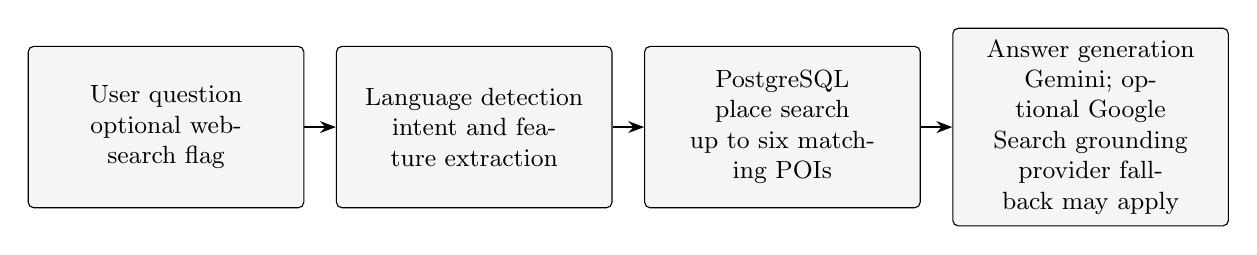
\begin{tikzpicture}[
        chatbox/.style={draw=black, fill=black!4, rounded corners=2pt,
            align=center, text width=3.2cm, minimum height=2.05cm,
            inner sep=1.5mm, font=\small},
        chatflow/.style={-{Stealth[length=2mm]}, thick, draw=black},
        node distance=4mm
    ]
        \node[chatbox] (question) {User question\\optional web-search flag};
        \node[chatbox, right=of question] (features) {Language detection\\intent and feature extraction};
        \node[chatbox, right=of features] (search) {PostgreSQL place search\\up to six matching POIs};
        \node[chatbox, right=of search] (answer) {Answer generation\\Gemini; optional Google Search grounding\\provider fallback may apply};
        \draw[chatflow] (question) -- (features);
        \draw[chatflow] (features) -- (search);
        \draw[chatflow] (search) -- (answer);
    \end{tikzpicture}
    \caption{Natural-language travel-search path and its conditional grounding step}
    \label{fig:chat_search_pipeline}
\end{figure}

The chat service is the path where current provider-based language generation is most visible. \url{travel_chatbot_service.py} includes a Gemini REST call, model fallback attempts, optional Google Search grounding, and a legacy OpenAI fallback. The exact path depends on keys, network access, provider responses, and the requested mode. The returned grounding metadata can include web queries and source URLs. These features should be described as conditional integrations: the repository alone does not show that credentials are set or prove that an external request succeeds in a deployed environment.

The chatbot search helper and the itinerary search tool are not interchangeable. The former uses extracted chat features and a search limit oriented to conversational responses. The latter takes explicit normalized itinerary parameters and searches \url{osm_attractions_staging} for planner candidates. A question answered by the chat function is not automatically stored as a travel plan.

\section{Itinerary Draft Workflow}

The itinerary API exposes both \url{/api/itinerary/plan-draft} and its alias \url{/api/itinerary/multi-agent/plan-draft}. The controller requires an ISO-formatted selected date and either a search term or coordinates. If an area label or location name is supplied without coordinates, the controller returns an input error: the source does not geocode the label in this path. When coordinates are provided, latitude and longitude must fall within a Vietnam bounding box, and the radius must be between 0.1 and 100 km. The default search radius for a coordinate-centered request is 5 km. The request also accepts a category, preferences, budget text, and a requested maximum stop count.

After input normalization, the controller calls \url{orchestrate_draft_itinerary()} with \code{execute\_api=False} and at most two retries. The orchestration sequence is:
\begin{enumerate}[leftmargin=1.8em,itemsep=3pt]
    \item Validate the request date, coordinate pair, radius, result limit, and stop count.
    \item Query PostgreSQL staging. If no candidates are found, return a clear not-found state rather than inventing POIs.
    \item Pass the candidate records to the planner. The default planner partitions candidates into dining-related and other POIs, then assigns selected records to a fixed sequence of day-time slots.
    \item Validate the draft against the original candidate list and geographic/time rules.
    \item If hard errors are present, feed them back and repeat, up to the configured retry limit. Warnings alone do not trigger another attempt.
    \item Return the final draft, validation report, route legs, warnings, candidate count, and iteration count. The API marks the result as unsaved.
\end{enumerate}

Figure~\ref{fig:itinerary_draft_pipeline} shows the draft route as sequential application logic. Validation errors can trigger a retry; warnings alone do not. The endpoint returns a draft without saving it.

\begin{figure}[htbp]
    \centering
    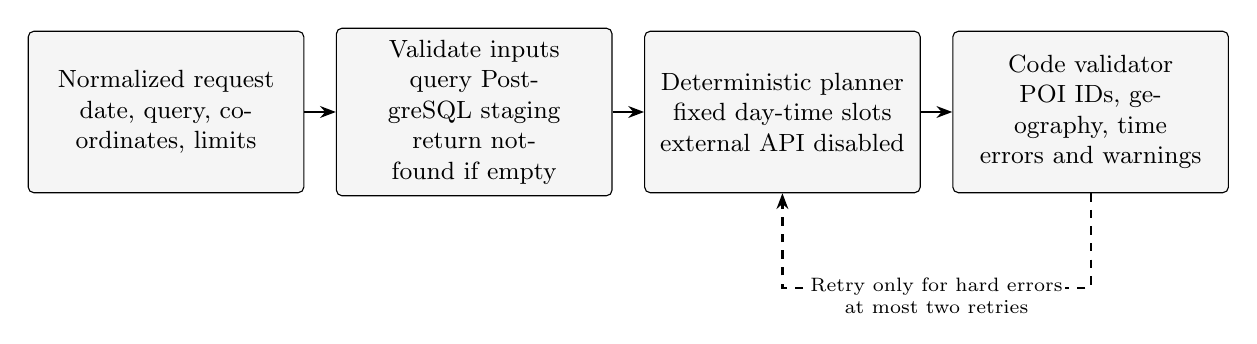
\begin{tikzpicture}[
        planbox/.style={draw=black, fill=black!4, rounded corners=2pt,
            align=center, text width=3.2cm, minimum height=2.05cm,
            inner sep=1.5mm, font=\small},
        planflow/.style={-{Stealth[length=2mm]}, thick, draw=black},
        retryflow/.style={-{Stealth[length=2mm]}, thick, dashed, draw=black},
        node distance=4mm
    ]
        \node[planbox] (request) {Normalized request\\date, query, coordinates, limits};
        \node[planbox, right=of request] (retrieve) {Validate inputs\\query PostgreSQL staging\\return not-found if empty};
        \node[planbox, right=of retrieve] (planner) {Deterministic planner\\fixed day-time slots\\external API disabled};
        \node[planbox, right=of planner] (validator) {Code validator\\POI IDs, geography, time\\errors and warnings};
        \draw[planflow] (request) -- (retrieve);
        \draw[planflow] (retrieve) -- (planner);
        \draw[planflow] (planner) -- (validator);
        \draw[retryflow] (validator.south) -- ++(0,-12mm) -| (planner.south);
        \node[font=\scriptsize, fill=white, inner sep=1pt, align=center]
            at ($(planner.south)!0.5!(validator.south)+(0,-13mm)$)
            {Retry only for hard errors\\at most two retries};
    \end{tikzpicture}
    \caption{Itinerary draft orchestration and validation feedback}
    \label{fig:itinerary_draft_pipeline}
\end{figure}

The schedule routine uses a fixed slot template rather than learning an itinerary policy. Its current slots begin at 08:30, 10:30, 12:30, 14:45, and 18:00, with durations from 90 to 120 minutes. It attempts to alternate dining and non-dining candidates according to slot labels, avoids reusing the same \code{osm\_id}, and limits the draft to the requested number of stops and available candidates. These are implementation details of the baseline engine; they are not evidence that the itinerary is globally optimal or personalized to a traveler.

The planner prompt builder and Gemini integration branch are present in \code{planner\_agent.py}. The optional branch requests structured JSON and uses a low-temperature configuration. However, the endpoint supplies \code{execute\_api=False}, so the planner uses \code{deterministic\_planner\_v1} on the default API path, regardless of whether a Gemini key happens to be configured. This distinction is central to interpreting any result from the current endpoint.\section{Validation and Route Estimates}

The validator separates blocking errors from warnings. It verifies that each draft stop references an OSM identifier present in the candidate set and that a stop is not duplicated. It checks that coordinates are numeric and fall inside the same broad Vietnam bounds used by the planner. It checks the \code{HH:MM} time format, requires the end to be after the start, reconciles declared duration with the time interval, and rejects overlapping visits. The total span from the first start to the last finish cannot exceed 12 hours.

Opening-hour validation is deliberately conditional. A simple hour range can be checked against a stop interval. A missing value produces a warning; a complex value that the simple parser cannot interpret also produces a warning for manual review. The validator does not claim to fully parse the OSM opening-hours grammar.

The routing helper computes Haversine distance between consecutive stops and multiplies it by 1.3. Each result is labeled as estimated, while \code{travel\_time\_minutes} is null. The Mapbox token helper reads a token from the environment, but the route function in the inspected implementation does not make a network request to Mapbox or OSRM. When no true drive duration exists, the validator reports that the time gap is undetermined instead of passing an estimate off as a route duration. The approximate distance is useful only as a coarse indication of spatial separation.

The implemented checks do not enforce the requested budget, even though the request can carry a budget value. They also do not optimize the stop order against road travel, calculate opening hours from a weekly calendar, consider transit schedules, or validate weather and event information. Those are current scope limits, not failed tests.

\section{Model and Provider Configuration}

The project has separate model/provider settings for the conversational answer path and the itinerary planner. Table~\ref{tab:model_configuration} summarizes configuration points visible in the source and environment loader. Credentials are read from environment variables; values are intentionally not reproduced in this report.

\begin{table}[htbp]
    \centering
    \caption{Provider and database settings visible in the source configuration}
    \label{tab:model_configuration}
    \renewcommand{\arraystretch}{1.2}
    \begin{tabularx}{\textwidth}{>{\raggedright\arraybackslash}p{3.7cm} >{\raggedright\arraybackslash}p{4.0cm} X}
        \toprule
        \textbf{Area} & \textbf{Configuration} & \textbf{Observed behavior} \\
        \midrule
        Chat response & \url{GEMINI_API_KEYS}, \url{GEMINI_API_KEY}, \url{GEMINI_MODEL} & Gemini REST integration tries a model pool; optional Google Search grounding is used when requested and supported. \\
        Chat fallback & \url{OPENAI_API_KEY} & Legacy OpenAI calls are present as a fallback path in the travel chat service. \\
        Draft planner & \url{GEMINI_API_KEYS}, \url{GEMINI_MODEL} & Gemini SDK branch exists, but the HTTP draft endpoint explicitly disables external API execution. \\
        Map routing & \code{MAPBOX\_ACCESS\_TOKEN} or \code{MAPBOX\_TOKEN} & Token accessor exists; itinerary routing currently returns a Haversine-based estimate. \\
        Database & \url{DATABASE_POSTGRESQL_URL} & SQLAlchemy uses PostgreSQL when a database URL is configured. \\
        Email & \code{MAIL\_SERVER}, \code{MAIL\_PORT}, TLS and account settings & Flask-Mail sends OTP and reminder messages when SMTP configuration is available. \\
        Authentication & \url{SECRET_KEY} & Used to sign and verify application JWTs. \\
        \bottomrule
    \end{tabularx}
\end{table}

The optional Gemini planner uses a structured JSON response request and a temperature of 0.2. Its default model string is \code{gemini-3-flash-preview}, but callers can override it through configuration. If the optional SDK or provider request fails, the planner falls back to the deterministic routine. The default HTTP route avoids this dependency by never enabling the API branch.

The travel-search service uses a different provider implementation. It creates REST requests to Gemini models with a configured temperature and output-token limit, retries through a model list, and can request a Google Search tool for non-JSON generation. It may use a legacy OpenAI call if the Gemini route is unavailable. These settings do not configure itinerary drafting because the planner endpoint is deliberately offline by default.

\section{Persistence, Accounts, and Supporting Services}

Draft creation and persistence are separate operations. The draft route returns an in-memory object and marks \code{is\_saved=False}. The confirmation endpoint is available at \url{/api/itinerary/confirm} and \url{/api/itinerary/multi-agent/confirm}. It requires a \code{draft\_id}, selected date, and non-empty items list, then derives the account identity from the Bearer JWT rather than trusting a user identifier in the request body. It verifies the token signature and expiry, looks up the user, and rejects unverified accounts. The confirmation service validates the request against staging data and commits the application itinerary through the relational model.

The account endpoints include registration, email verification with a one-time code, login, password-reset steps, and username update. The user model stores a password hash rather than a plaintext password. The chat models store conversations and messages; itinerary entities link the user, trip date, and ordered attraction visits. Notifications can be queried, marked read, and deleted through their own namespace.

The application factory calls \code{db.create\_all()} inside an app context, but catches connection errors and logs a warning. The repository also provides SQL migrations for the OSM staging and notifications tables. This combination supports local development, but it does not constitute a versioned migration framework for every model change; deployment procedures should apply and verify migrations explicitly.

The scheduler in \code{scheduler\_service.py} is started when \code{main.py} runs. It periodically checks upcoming itineraries and calls the email service. The development entry point enables Flask debug mode and binds to localhost. That is appropriate for local use but should be changed for production deployment. The Docker Compose file provides a PostgreSQL-compatible development container using the pgvector image, but the itinerary query path described here uses relational columns and does not require vector-extension operations.

\section{Security and Operational Considerations}

The project reads database, mail, model, map, and signing credentials from environment configuration. The report does not expose local \code{.env} values. A deployment should keep the environment file outside source control, rotate any credentials that have been exposed, use a strong signing key, and limit access to the database. HTTP provider integrations introduce cost, rate-limit, availability, and data-transfer considerations. User questions can contain personal context, so provider calls should be disclosed and minimized according to the deployment's privacy requirements.

The confirmation flow has a useful identity boundary: the server derives the user from the signed token and does not accept the request body's \code{user\_id} as authority. Still, token, OTP, registration, and password-reset behavior should be independently reviewed for expiry, rate limiting, brute-force protection, and secure transport before public deployment. Database connection success, migration status, provider availability, and SMTP delivery should be observable with structured logs that exclude secrets and unnecessary personal content.

SQLAlchemy parameters are used for the itinerary search values, and the staging migration declares a unique constraint on \code{osm\_id} plus indexes for coordinates, category, feature class, source layer, and import status. These support expected retrieval and idempotent ingestion patterns. Performance at scale remains unmeasured in the repository snapshot and must be tested against a provisioned database with recorded hardware and configuration.

\section{Development Configuration}

The local setup described by the repository creates a Python virtual environment, installs \code{requirements.txt}, starts the development database with \code{docker compose -f docker-compose.dev.yml up -d}, configures required environment variables, applies the relevant SQL migration, imports the POIs with an explicit \code{--apply} flag, and starts the server with \code{python main.py}. The developer interface is available at the root path and Swagger documentation at \code{/docs}.

Because the importer defaults to dry run and the draft endpoint defaults to deterministic offline execution, the core dataset-processing and itinerary-drafting path can be developed without model-provider API calls. Database-backed behavior still requires a reachable PostgreSQL instance with the staging table available. Optional chatbot generation, SMTP, and map services require their respective credentials and network access.

\chapter{Experimental Results and Discussion}
\label{chap:results_discussion}

\section{Evaluation Scope and Evidence Available}

A quantitative evaluation should be grounded in a fixed dataset, labeled queries, a defined system configuration, and recorded execution output. The repository snapshot contains a data-processing summary, a small pilot fixture, implementation code, and a test module. The existing nine-case unittest suite was executed against the current local working tree; the recorded run is summarized below. The project still does not contain a labeled POI retrieval benchmark, a response-quality annotation set, output logs from an LLM evaluation, or a reproducible load-test report. This chapter therefore reports the completed regression run and other available evidence, while describing a protocol for collecting the missing model and system measurements.

The distinction matters because three types of statement are often confused. First, a source-code rule (for example, rejecting a repeated \code{osm\_id}) is an implemented behavior. Second, an executed unit-test result provides evidence that selected assertions passed for the tested local working tree. Third, a model metric such as answer accuracy or route feasibility requires a defined test corpus and measured outputs. The run below supports limited regression claims; it does not document the third type of evidence.

The proposed evaluation separates three tracks so that retrieval, schedule feasibility, and answer grounding are measured independently. Figure~\ref{fig:evaluation_protocol} summarizes the evidence needed; it does not represent completed experiments.

\begin{figure}[htbp]
    \centering
    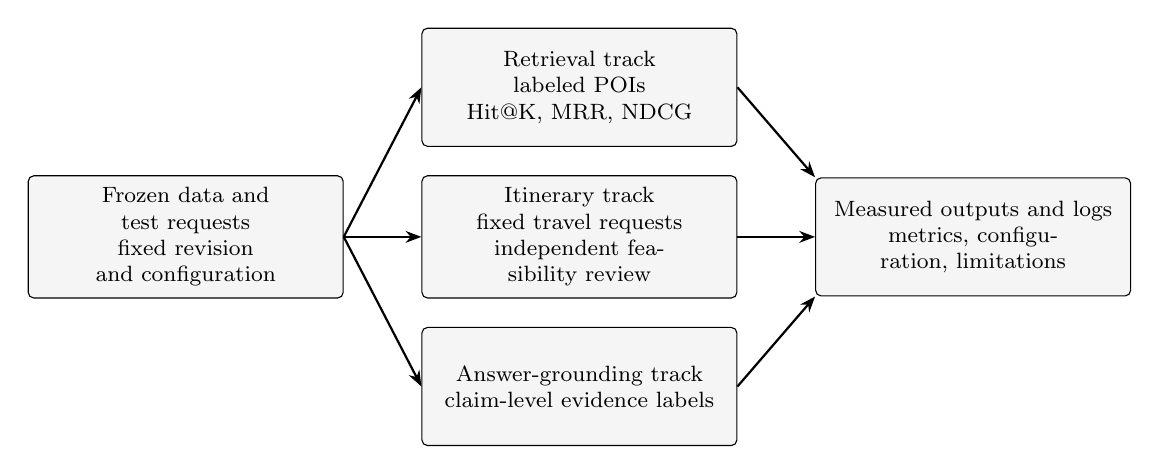
\begin{tikzpicture}[
        evalbox/.style={draw=black, fill=black!4, rounded corners=2pt,
            align=center, text width=3.7cm, minimum height=1.5cm,
            inner sep=1.5mm, font=\footnotesize},
        evalflow/.style={-{Stealth[length=2mm]}, thick, draw=black}
    ]
        \node[evalbox] (inputs) at (0,0) {Frozen data and test requests\\fixed revision and configuration};
        \node[evalbox] (retrieval) at (5,1.9) {Retrieval track\\labeled POIs\\Hit@K, MRR, NDCG};
        \node[evalbox] (planning) at (5,0) {Itinerary track\\fixed travel requests\\independent feasibility review};
        \node[evalbox] (answers) at (5,-1.9) {Answer-grounding track\\claim-level evidence labels};
        \node[evalbox] (report) at (10,0) {Measured outputs and logs\\metrics, configuration, limitations};
        \draw[evalflow] (inputs.east) -- (retrieval.west);
        \draw[evalflow] (inputs.east) -- (planning.west);
        \draw[evalflow] (inputs.east) -- (answers.west);
        \draw[evalflow] (retrieval.east) -- (report.north west);
        \draw[evalflow] (planning.east) -- (report.west);
        \draw[evalflow] (answers.east) -- (report.south west);
    \end{tikzpicture}
    \caption{Recommended evaluation evidence flow; labeled retrieval, itinerary-quality, answer-grounding, and runtime benchmark results remain unavailable}
    \label{fig:evaluation_protocol}
\end{figure}

\section{Dataset Processing Results}

The committed processing summary records 110,421 input records across the three imported layers. Of these, 30,941 rows pass layer-level candidate filtering and 30,839 unique identifiers are listed after deduplication. The summary provides category counts and layer-level rejection counts, reproduced in Chapter~\ref{chap:dataset}. Those values are useful as a descriptive data profile and show that the import pipeline performs substantial name/class/coordinate filtering.

The manifest's counts are not fully self-consistent. Subtracting 30,839 unique IDs from 30,941 candidates gives 102 duplicate rows, whereas the explicit duplicate field reports 100. The grouped category counts do sum to 30,839. This inconsistency is a data-quality finding, not a corrected result. A fresh import audit should emit each duplicate OSM ID and the source layers in which it occurs, then reconcile the summary before presenting a final accepted-row count.

The summary lists null values for unknown price, rating, and opening hours, and defines a coordinate-based fallback address. This is a positive design choice because the data pipeline does not substitute made-up values. The trade-off is that the catalogue's usefulness varies by field: a point can be geographically searchable while lacking the details needed to answer whether it is open, affordable, or appropriate for a visit. The repository does not publish field-level completeness percentages, so completeness rates cannot be calculated from the evidence reviewed.

\section{Functional Test Design in the Repository}

The file \code{tests/test\_multi\_agent\_flow.py} defines nine unittest methods. Its module docstring states that the tests use the pilot fixture and mocked database/provider calls and do not connect to or write to the configured PostgreSQL database. Table~\ref{tab:declared_tests} summarizes the assertions represented by those methods and their outcomes in the recorded local run.

\begin{table}[htbp]
    \centering
    \caption{Regression test cases and outcomes in the recorded local run}
    \label{tab:declared_tests}
    \renewcommand{\arraystretch}{1.15}
    \begin{tabularx}{\textwidth}{c >{\raggedright\arraybackslash}p{4.4cm} >{\raggedright\arraybackslash}X c}
        \toprule
        \textbf{No.} & \textbf{Test scenario} & \textbf{Expected behavior encoded by the assertion} & \textbf{Run} \\
        \midrule
        1 & Offline planner with flat pilot coordinates & Successful validated draft, three stops, and non-null latitude and longitude values & PASS \\
        2 & Plan-draft endpoint with mocked POI results & HTTP 200, valid draft, and \code{is\_saved=False} & PASS \\
        3 & Invalid selected-date text & HTTP 400 & PASS \\
        4 & Date in the past & HTTP 400 and invalid-request status & PASS \\
        5 & Latitude without longitude & HTTP 400 & PASS \\
        6 & Non-numeric coordinate input & HTTP 400 & PASS \\
        7 & Simulated staging database error & HTTP 503 and database-error status & PASS \\
        8 & Confirm endpoint without Bearer token & HTTP 401 & PASS \\
        9 & Login with mocked auth service & HTTP 200 and the mocked token/user payload & PASS \\
        \bottomrule
    \end{tabularx}
\end{table}

These cases target input validation, the offline planning path, API status mapping, and selected authentication behavior. The test module does not exercise a live PostgreSQL connection, actual transaction rollback, email delivery, an external language-model provider, Google Search grounding, actual road routing, or concurrent load. It does not score response relevance or truthfulness. The passing run is useful regression evidence, but it is not evidence of production reliability or model quality.

The run was performed on 21 October 2026 from the repository root using Python 3.10.11 from the project virtual environment. The command was \code{venv/Scripts/python.exe -m unittest discover -s tests -p test\_*.py -v}; the runner reported \code{Ran 9 tests in 0.048s; OK}. All nine cases in Table~\ref{tab:declared_tests} passed, with zero failures and zero errors. The checkout contained uncommitted changes, so this result applies to the local working tree at the time of execution rather than to a clean tagged release. Database and provider calls were mocked; the runtime is the duration of this small unit-test suite, not an application latency benchmark.

\section{Implemented Behavior Observed by Source Inspection}

Several properties can be established from the implementation without claiming benchmark results:
\begin{itemize}[leftmargin=1.8em,itemsep=3pt]
    \item The itinerary endpoint sets \code{execute\_api=False}; its normal draft path therefore uses the deterministic scheduling routine.
    \item The orchestrator passes only database-retrieved or explicitly supplied candidate POIs to the planner, and the validator checks draft identifiers against that candidate set.
    \item The route helper returns a Haversine-based distance estimate multiplied by 1.3 and leaves travel time unknown.
    \item The validator separates errors that invalidate a draft from warnings about missing or complex opening-hour information and unknown travel time.
    \item The draft endpoint returns an unsaved object. Confirmation is a separate operation guarded by a verified-user JWT lookup.
    \item The radius search performs a bounding-box prefilter, exact Haversine radius check, distance ordering, and then limiting.
\end{itemize}

These properties explain the software's safety boundaries, but they do not quantify their real-world effectiveness. For example, checking that a drafted \code{osm\_id} belongs to the candidate set prevents a planner from adding an identifier outside that set. It does not verify that an OSM name is accurate, that a POI is still operating, or that the candidate set itself contains the best locations.

\section{Proposed Retrieval Evaluation}

A future retrieval study should begin with a manually labeled query set. Each query should have one or more relevant OSM IDs and a reason for relevance, with categories covering exact place names, categories, text-only area labels, coordinate-centered searches, Vietnamese diacritics, and multilingual wording. Each query should be run against a frozen database snapshot and a recorded limit and radius. The relevance label must be prepared independently of the search results to avoid scoring the system against its own output.

For a query set $\mathcal{Q}$, the following ranking measures are suitable:
\begin{align}
    \operatorname{Hit@K}
    &= \frac{1}{|\mathcal{Q}|}
       \sum_{q\in\mathcal{Q}}
       \mathbb{I}\left(R_q^{(K)}\cap G_q\ne\varnothing\right),\\
    \operatorname{MRR}
    &= \frac{1}{|\mathcal{Q}|}
       \sum_{q\in\mathcal{Q}}\frac{1}{\operatorname{rank}_q},\\
    \operatorname{NDCG@K}
    &= \frac{\operatorname{DCG@K}}{\operatorname{IDCG@K}},
\end{align}
where $R_q^{(K)}$ is the retrieved top-$K$, $G_q$ is the set of relevant IDs, and $\operatorname{rank}_q$ is the first relevant position. Hit@K measures whether at least one known relevant item appears; MRR rewards earlier first relevant results; NDCG accommodates graded relevance when annotators distinguish exact, close, and weak matches. None of these scores is available in the current snapshot.

At minimum, a retrieval evaluation should compare the current SQL text/category search against a geographic-only baseline and a clearly specified semantic-search baseline if the optional Chroma index is intended for deployment. All approaches must use the same frozen catalogue and query set. Results should be reported by query type and language, since an aggregate score can conceal poor performance on local names, administrative labels, or non-Vietnamese queries. A ranking score alone should not be interpreted as factual response accuracy.

\section{Proposed Itinerary and Answer Evaluation}

For itinerary drafts, a useful primary measure is the independently audited feasibility rate:
\begin{equation}
    \operatorname{FeasibilityRate}
    = \frac{\text{drafts meeting all predefined hard constraints}}
           {\text{drafts reviewed}}.
\end{equation}
The hard-constraint checklist should include candidate-set membership, duplicate stops, coordinate validity, valid time intervals, interval overlap, daily span, and any enforceable opening-hour rules. Because the validator implements only a subset of real travel constraints, a human audit or independent checker should also consider route plausibility, accessibility, opening calendars, and available time. A validator's own \code{valid=True} output cannot serve as the sole ground truth for measuring that validator.

Grounded answer quality should be assessed at the claim level. Reviewers can label each factual claim as supported by the retrieved OSM record, supported by a cited web source, unsupported, or contradicted. This makes it possible to distinguish a correct place name from a fabricated price or an unqualified opening-hour statement. Human ratings of relevance, clarity, and language quality can supplement automated text similarity. BLEU and ROUGE are available as established text-overlap measures \cite{papineni2002bleu,lin2004rouge}, but are insufficient by themselves for open-ended travel advice: a faithful paraphrase may have low overlap, while a fluent answer may repeat reference words and still contain a false claim.

Route evaluation requires a reference routing source and a declared travel mode. For each stop pair, the system's estimated distance can be compared with a road-network distance and the error distribution reported. Since the current route helper returns no estimated duration, travel-time error cannot yet be calculated for the default itinerary path. If a road-routing API is integrated, evaluation should record its date, mode, avoidances, and API version because these affect routes and traffic assumptions.

\section{Proposed Runtime and Reliability Evaluation}

No latency, throughput, provider error, or load-test measurements are included in the repository snapshot. A reproducible runtime study should name the host CPU/RAM, Python version, dependency lock, PostgreSQL version and row count, network conditions, model/provider and region, concurrency schedule, warm-up duration, and total request count. It should separate database-only search, deterministic draft generation, live provider-backed generation, and confirmation transactions. Those routes have different cost and latency profiles and should not be aggregated into one number.

For each endpoint and concurrency level, report median and 95th-percentile latency, completed requests per second, status-code counts, timeout rate, database pool saturation if configured, and external-provider failures. Repeat each run and report variability. A load test against a mocked model does not establish the behavior of an external provider, and a local developer server with Flask debug enabled is not representative of a production WSGI deployment.

\section{Discussion of Current Results}

The available evidence supports a modest conclusion. The data-preparation summary describes a broad filtered candidate set; the SQL model and query tool provide a concrete geographic search mechanism; the draft planner has a deterministic offline execution path; and the validator encodes several useful structural and temporal safeguards. A safe, mocked regression suite is present for representative request and response cases. This is meaningful implementation evidence for a capstone prototype.

The evidence does not support the numerical claims found in the earlier draft of this report about retrieval hit rate, multilingual BLEU/ROUGE scores, itinerary feasibility percentages, zero hallucination, or concurrent throughput. The repository contains no corresponding labeled test set or run log. Such values have been removed from the report rather than reused as if they were measured. Similarly, the presence of \code{chromadb}, \code{sentence-transformers}, and \code{pgvector} in dependencies or the container image does not establish a working vector retrieval benchmark in the default itinerary flow.

Several implementation constraints directly affect interpretation:
\begin{enumerate}[leftmargin=1.8em,itemsep=3pt]
    \item \textbf{Planner personalization is limited.} The baseline uses a fixed slot schedule and coarse dining classification. User preference and budget fields are accepted but not comprehensively scored or validated.
    \item \textbf{Retries may not improve the draft.} The orchestrator can return validator feedback for up to two retries. The deterministic selection routine does not perform an explicit search over alternatives in response to each error, so retries are a control-flow feature whose practical value should be tested.
    \item \textbf{Road feasibility remains unknown.} Approximate distances are reported without drive times. Time gaps between visits cannot be certified as sufficient for travel in the default path.
    \item \textbf{Data freshness and detail vary.} Null hours and prices limit concrete guidance; a count of records does not establish that records are current or tourism-relevant.
    \item \textbf{The manifest has an unresolved count mismatch.} A release-level import audit is needed to reconcile duplicate rows and verify the deployed staging-table count.
\end{enumerate}

\section{Recommended Evaluation Sequence}

The next evaluation cycle should proceed in an order that limits confounding:
\begin{enumerate}[leftmargin=1.8em,itemsep=3pt]
    \item Rerun the importer in dry-run mode from the checked-in OSM extract; produce per-layer counts, an explicit duplicate-ID file, and a reconciled final count.
    \item Load a frozen copy into a test PostgreSQL database, record the schema version, and query total rows and field completeness.
    \item Preserve the recorded unittest outcome with the exact checkout state. Then add direct tests for validator boundary conditions and confirm-service transaction behavior, and rerun the suite after each relevant code change.
    \item Create a blinded, manually labeled query set and score text, category, and radius retrieval separately.
    \item Evaluate deterministic itinerary drafts on a fixed request set. Compare validator output with an independent human or reference-rule audit, and report each constraint separately.
    \item Evaluate the provider-backed chat and planner only after recording model names, prompts, parameters, provider region, and exact request/response outputs under a privacy-safe protocol.
    \item Conduct performance and failure testing against a production-like WSGI process and database, reporting the configuration alongside all latency and error results.
\end{enumerate}

\section{Chapter Summary}

The current report records descriptive data-processing figures, concrete source-level behavior, and one successful local run of the nine-case regression suite (9 passed, 0 failed, 0 errors). Because database and provider calls were mocked, this run does not establish live integration, model quality, or production reliability. The strongest defensible system result remains that a database-grounded, offline draft-and-validation workflow is implemented with explicit uncertainty around missing opening hours and road travel time. The main empirical work still needed is to verify the imported dataset, measure retrieval relevance, independently audit itinerary feasibility, and benchmark each runtime path separately.


\clearpage
\printbibliography[heading=bibintoc,title={References}]

\clearpage
\appendix

\chapter{Data Dictionary and Reproducibility Notes}
\label{app:data}

\section{Staging Record Fields}

The OSM staging model preserves a source-facing record rather than pretending every OSM feature has the detail of a curated attraction. Table~\ref{tab:staging_dictionary} describes the key columns defined by \code{OsmAttractionStaging} and the staging migration.

\begin{longtable}{>{\raggedright\arraybackslash}p{3.3cm} >{\raggedright\arraybackslash}p{3.0cm} >{\raggedright\arraybackslash}p{7.0cm}}
\caption{OSM staging field dictionary}\\
\label{tab:staging_dictionary}\\
\toprule
\textbf{Field} & \textbf{Type / constraint} & \textbf{Meaning} \\
\midrule
\endfirsthead
\toprule
\textbf{Field} & \textbf{Type / constraint} & \textbf{Meaning} \\
\midrule
\endhead
\code{id} & Integer primary key & Internal staging row identifier. \\
\code{osm\_id} & String, unique, not null & Stable source feature identifier used for deduplication and traceability. \\
\code{osm\_source\_layer} & String, not null & Name of the source shapefile layer. \\
\code{osm\_code} & Integer, optional & Numeric source class code when available. \\
\code{fclass} & String, not null & Original OSM feature class. \\
\code{name} & String, not null & Display name retained from the source record. \\
\code{category} & String, not null & Normalized travel-facing category. \\
\code{latitude}, \code{longitude} & Double precision, not null & Geographic coordinates in WGS 84 decimal degrees. \\
\code{address} & String, not null & Source address when available; otherwise explicit coordinate-based fallback text. \\
\code{description} & Text, optional & Brief description derived from retained OSM information. \\
\code{price}, \code{rating} & Numeric, optional & Unknown values remain null in the import standard. \\
\code{opening\_hours} & String, optional & OSM hours string; format may be complex or absent. \\
\code{phone\_number}, \code{image\_url} & String, optional & Contact and image metadata when present. \\
\code{language} & String & Language label assigned by the import process. \\
\code{tags}, \code{aliases} & JSONB & Searchable tags and alternative names. \\
\code{raw\_properties} & JSONB & Original property values retained for traceability. \\
\url{imported_to_attraction}, \url{attraction_id} & Boolean and string & Promotion state and optional link to the core application attraction. \\
\code{created\_at}, \code{updated\_at} & Timestamp & Row creation and update times. \\
\bottomrule
\end{longtable}

\section{Import Reproduction Checklist}

The repository's import script is designed to support a dry-run review before writes are enabled. A release record should include:
\begin{enumerate}[leftmargin=1.8em,itemsep=3pt]
    \item the extract timestamp and license notice from the source package;
    \item file checksums for the three input layers;
    \item the exact Python version and installed dependency versions;
    \item importer options, including deduplication mode and batch size;
    \item raw row counts, per-filter rejection counts, and retained counts by layer;
    \item a machine-readable duplicate report listing each repeated OSM identifier;
    \item a final staging row count and a sample of records queried from PostgreSQL;
    \item the database schema or migration revision used for the load.
\end{enumerate}
This checklist would resolve the current ambiguity between the summary's candidate, unique, and duplicate counts. A safe release should also retain the dry-run report alongside the applied-run report so that proposed changes can be compared with actual writes.

\chapter{API Surface and Request Boundaries}
\label{app:api}

\section{Core Travel and Itinerary Routes}

Table~\ref{tab:core_api} summarizes the routes central to the project topic. The route paths and operation purpose are derived from the registered Flask-RESTX namespaces and controllers. The interactive Swagger page at \code{/docs} is the primary runtime reference for detailed schemas and status responses.

\begin{longtable}{>{\raggedright\arraybackslash}p{2.3cm} >{\raggedright\arraybackslash}p{5.0cm} >{\raggedright\arraybackslash}p{6.0cm}}
\caption{Core travel-search and itinerary endpoints}\\
\label{tab:core_api}\\
\toprule
\textbf{Method} & \textbf{Path} & \textbf{Purpose / boundary} \\
\midrule
\endfirsthead
\toprule
\textbf{Method} & \textbf{Path} & \textbf{Purpose / boundary} \\
\midrule
\endhead
POST & \url{/api/travel-chatbot/search} & Accepts a natural-language travel question and an optional web-search flag; returns search results and a generated response. \\
GET & \url{/api/travel-chatbot/metadata} & Reads paginated place metadata through the travel-chatbot controller. \\
GET & \url{/api/travel-chatbot/embeddings} & Legacy embeddings route retained in the controller; it is not the default itinerary retrieval mechanism. \\
POST & \url{/api/itinerary/plan-draft} & Generates a draft. Requires a selected date and either a text query or a valid coordinate pair; does not persist the draft. \\
POST & \url{/api/itinerary/multi-agent/plan-draft} & Alias for the draft-planning operation. \\
POST & \url{/api/itinerary/confirm} & Confirms and persists a draft using the verified account from a Bearer JWT. \\
POST & \url{/api/itinerary/multi-agent/confirm} & Alias for the confirmation operation. \\
GET / POST / DELETE & \url{/api/itinerary/...} & Existing list, detail, create, delete, and item-update operations for persisted itineraries. Consult Swagger for the exact method and payload of each resource. \\
\bottomrule
\end{longtable}

\section{Draft Request Validation}

The plan-draft controller accepts a date, optional free-text query, destination or area label, category, coordinates, radius, preferences, budget, maximum stop count, and an optional user prompt. It rejects a partial coordinate pair, non-numeric or out-of-range coordinates, a radius outside the supported interval, and an area label without a coordinate center. This last rule is important: the itinerary controller does not translate an area name into a coordinate.

The orchestrator further validates request-level limits, including a stop count from one through ten and a search result limit from one through one hundred. A date in the past is rejected in the orchestration layer. Search failures are mapped to explicit response statuses; database unavailability is reported separately from invalid input and a valid empty search.

\section{Draft Confirmation Boundary}

The confirmation route requires a draft identifier in the form expected by its controller, a selected date, and a non-empty list of itinerary items. It reads the Bearer token from the authorization header, verifies its signature and expiry, obtains the authenticated user, and checks that the user's email is verified. A user identifier included in the JSON body is not accepted as the authority for ownership.

The confirmation service rechecks draft details against staging records and persists a relational itinerary. A successful new confirmation returns HTTP 201; a recognized duplicate request can return HTTP 200. Validation errors, missing data, authorization failures, and transaction errors are represented by distinct response categories. These controller-level response codes are part of the API contract and should remain stable if the planning implementation changes.\chapter{Regression Test and Evaluation Register}
\label{app:evaluation}

\section{Existing Regression Cases}

The nine test methods in \url{tests/test_multi_agent_flow.py} form a compact offline regression layer. The fixture contains 15 OSM-shaped records and allows planner behavior to be exercised without a production database. Provider and database functions are patched where the test needs to isolate controller behavior. This suite was executed from the repository root in the project virtual environment; the recorded result is provided below. It did not rely on or write to a user's live database.

\begin{longtable}{c >{\raggedright\arraybackslash}p{4.4cm} >{\raggedright\arraybackslash}p{7.4cm} c}
\caption{Test-to-requirement mapping and observed outcomes}\\
\label{tab:test_mapping}\\
\toprule
\textbf{ID} & \textbf{Requirement area} & \textbf{Assertion represented in the source} & \textbf{Run} \\
\midrule
\endfirsthead
\toprule
\textbf{ID} & \textbf{Requirement area} & \textbf{Assertion represented in the source} & \textbf{Run} \\
\midrule
\endhead
T-01 & Offline planning & The planner returns a successful valid draft with three stops and non-null latitude/longitude values. & PASS \\
T-02 & Draft API contract & A mocked staging search produces HTTP 200 and a response marked unsaved. & PASS \\
T-03 & Input validation & An invalid date string is rejected with HTTP 400. & PASS \\
T-04 & Input validation & A past selected date is rejected with HTTP 400. & PASS \\
T-05 & Coordinate validation & Supplying latitude without longitude is rejected with HTTP 400. & PASS \\
T-06 & Coordinate validation & Non-numeric coordinate values are rejected with HTTP 400. & PASS \\
T-07 & Failure mapping & A mocked staging database error maps to HTTP 503. & PASS \\
T-08 & Confirmation authorization & A confirmation request without a Bearer token maps to HTTP 401. & PASS \\
T-09 & Login controller & A mocked authentication service response is returned as HTTP 200 with token and user fields. & PASS \\
\bottomrule
\end{longtable}

The recorded run took place on 21 October 2026 with Python 3.10.11 from the project virtual environment. The command was \code{venv/Scripts/python.exe -m unittest discover -s tests -p test\_*.py -v}; the runner reported \code{Ran 9 tests in 0.048s; OK}. All cases T-01 through T-09 passed, with zero failures and zero errors. The working tree contained uncommitted changes, so the outcome applies to that local snapshot and does not guarantee later revisions. Database and provider calls were mocked. Future runs should record their exact checkout state and output; logs must not include tokens, passwords, personal user records, or sensitive provider payloads.

\section{Additional Tests Recommended Before Release}

The current tests focus on happy-path draft creation and several request boundaries. A broader regression suite should cover these areas:
\begin{itemize}[leftmargin=1.8em,itemsep=3pt]
    \item \textbf{Search correctness:} compare SQL radius results with an independent Haversine calculation; verify nearest-first order and ensure the limit is applied after radius filtering.
    \item \textbf{Data ingestion:} test duplicate IDs across and within layers, malformed coordinates, empty names, category mappings, null preservation, and upsert idempotency against a disposable database.
    \item \textbf{Validator boundaries:} test midnight edge cases, malformed time values, zero-length visits, overlap at equality, the 12-hour maximum, simple opening-hour ranges, complex hours, and missing coordinates.
    \item \textbf{Planner semantics:} verify uniqueness, stop-count limits, candidate coverage, deterministic output for a fixed fixture, and behavior when dining or sightseeing categories are absent.
    \item \textbf{Retries:} construct a candidate set that triggers a hard error and verify whether feedback changes the second attempt or merely repeats the original plan.
    \item \textbf{Persistence:} verify that confirmation revalidates current staging data, maps OSM IDs to core attractions, assigns the authenticated user, and rolls back all writes on a forced failure.
    \item \textbf{Provider integration:} use provider mocks to test malformed structured output, quota responses, timeout, fallback, missing credentials, and safety of logs.
    \item \textbf{Access control:} test expired, malformed, and tampered JWTs; unverified users; attempts to confirm another user's draft; and OTP expiry and rate limits.
\end{itemize}

\section{Evaluation Record Template}

When measurements are collected, the results table should include enough context to be independently interpreted. Table~\ref{tab:evaluation_record} is a blank record template, not a report of completed measurements.

\begin{table}[htbp]
    \centering
    \caption{Evaluation record template for a future run}
    \label{tab:evaluation_record}
    \renewcommand{\arraystretch}{1.3}
    \begin{tabularx}{\textwidth}{>{\raggedright\arraybackslash}p{4.0cm} X}
        \toprule
        \textbf{Field} & \textbf{Value to record} \\
        \midrule
        Source revision & Git commit or archive identifier \\
        Dataset version & OSM extract timestamp, file checksums, final database row count \\
        Environment & OS, CPU, memory, Python and PostgreSQL versions \\
        Provider settings & Model ID, region, temperature, output limit, grounding mode, prompt revision \\
        Query set & Number of queries, languages, category mix, annotation procedure \\
        Search metrics & Hit@K, MRR, NDCG by language, category, and location-query type \\
        Itinerary metrics & Independent feasibility rate and per-constraint violations \\
        Answer review & Supported factual claims, unsupported claims, relevance and clarity ratings \\
        Runtime metrics & p50 / p95 latency, throughput, error and timeout rates by endpoint \\
        Repetitions & Number of independent runs and variance or confidence interval method \\
        Limitations & Missing labels, provider outages, data gaps, and deviations from protocol \\
        \bottomrule
    \end{tabularx}
\end{table}

\section{Local Development Commands}

The project README describes the following broad development sequence. Commands should be run from the repository root, after local environment values have been configured:

\begin{lstlisting}[language=bash,caption={Local development sequence documented by the project}]
python -m venv venv
pip install -r requirements.txt
docker compose -f docker-compose.dev.yml up -d
python scripts/import_all_osm_poi.py --apply --batch-size 1000
python main.py
\end{lstlisting}

The importer should first be run without \code{--apply} when reviewing a new source extract. The current repository's migrations should be checked and applied before the import. The development server should not be exposed publicly with debug mode enabled. For reproducible experiments, capture command output and configuration metadata separately from secrets.

\section{Closing Note}

This register is intended to make the report's evidence boundary easy to audit. The current report records a dataset summary and a passing nine-case local regression run. Future labeled evaluations and live integration/performance runs should be added with versions and methodology, then used to replace planned metrics with measured results. Until those records exist, numerical model-quality or throughput claims should remain out of the final report.


\clearpage
\clearpage
\chapter*{6. Instructor Review and Comment}
\addcontentsline{toc}{chapter}{6. Instructor Review and Comment}

{\renewcommand{\thetable}{6.1}%
\captionof{table}{Capstone Project Evaluation Rubric and Instructor Feedback}\label{tab:instructor_rubric}}

\renewcommand{\arraystretch}{1.55}
\noindent\begin{tabularx}{\textwidth}{|>{\raggedright\arraybackslash}p{4.2cm}|>{\centering\arraybackslash}p{1.8cm}|>{\raggedright\arraybackslash}X|}
    \hline
    \rowcolor{SamsungLightBlue}
    \textbf{CATEGORY} & \textbf{SCORE} & \textbf{REVIEW AND COMMENT} \\
    \hline
    IDEA & \rule{0.7cm}{0.4pt}/10 & \\
    \hline
    APPLICATION & \rule{0.7cm}{0.4pt}/30 & \\
    \hline
    RESULT & \rule{0.7cm}{0.4pt}/30 & \\
    \hline
    PROJECT MANAGEMENT & \rule{0.7cm}{0.4pt}/10 & \\
    \hline
    PRESENTATION AND REPORT & \rule{0.7cm}{0.4pt}/20 & \\
    \hline
    \rowcolor{SamsungLightBlue}
    \textbf{TOTAL} & \rule{0.7cm}{0.4pt}/100 & \\
    \hline
\end{tabularx}

\vspace{1.2cm}
\noindent\begin{minipage}[t]{0.56\textwidth}
    \centering Instructor Signature\\[1.2cm]
    \rule{0.82\linewidth}{0.4pt}
\end{minipage}\hfill
\begin{minipage}[t]{0.36\textwidth}
    \centering Date\\[1.2cm]
    \rule{0.82\linewidth}{0.4pt}
\end{minipage}

\vspace{0.8cm}
\begin{center}
    \textbf{TS. Trần Quang Quý}
\end{center}


\end{document}
